%%%%%%%%%%%%%%%%%%%%%%%%%%%%%%%%%%%
%This is the LaTeX ARTICLE template for RSC journals
%Copyright The Royal Society of Chemistry 2016
%%%%%%%%%%%%%%%%%%%%%%%%%%%%%%%%%%%

\documentclass[twoside,twocolumn,9pt]{article}
\usepackage{extsizes}
\usepackage[super,sort&compress,comma]{natbib} 
\usepackage[version=3]{mhchem}
\usepackage[left=1.5cm, right=1.5cm, top=1.785cm, bottom=2.0cm]{geometry}
\usepackage{balance}
\usepackage{times,mathptmx}
\usepackage{sectsty}
\usepackage{graphicx} 
\usepackage{lastpage}
\usepackage[format=plain,justification=justified,singlelinecheck=false,font={stretch=1.125,small,sf},labelfont=bf,labelsep=space]{caption}
\usepackage{float}
\usepackage{fancyhdr}
\usepackage{fnpos}
\usepackage[english]{babel}
\usepackage{array}
\usepackage{droidsans}
\usepackage{charter}
\usepackage[T1]{fontenc}
\usepackage[usenames,dvipsnames]{xcolor}
\usepackage{setspace}
\usepackage[compact]{titlesec}
%%%Please don't disable any packages in the preamble, as this may cause the template to display incorrectly.%%%
\usepackage[obeyFinal]{easy-todo}
\usepackage{url}
\usepackage{rotating}

\usepackage{epstopdf}%This line makes .eps figures into .pdf - please comment out if not required.

\definecolor{cream}{RGB}{222,217,201}

\begin{document}

\pagestyle{fancy}
\thispagestyle{plain}
\fancypagestyle{plain}{

%%%HEADER%%%
\fancyhead[C]{\includegraphics[width=18.5cm]{head_foot/header_bar}}
\fancyhead[L]{\hspace{0cm}\vspace{1.5cm}\includegraphics[height=30pt]{head_foot/journal_name}}
\fancyhead[R]{\hspace{0cm}\vspace{1.7cm}\includegraphics[height=55pt]{head_foot/RSC_LOGO_CMYK}}
\renewcommand{\headrulewidth}{0pt}
}
%%%END OF HEADER%%%

%%%PAGE SETUP - Please do not change any commands within this section%%%
\makeFNbottom
\makeatletter
\renewcommand\LARGE{\@setfontsize\LARGE{15pt}{17}}
\renewcommand\Large{\@setfontsize\Large{12pt}{14}}
\renewcommand\large{\@setfontsize\large{10pt}{12}}
\renewcommand\footnotesize{\@setfontsize\footnotesize{7pt}{10}}
\makeatother

\renewcommand{\thefootnote}{\fnsymbol{footnote}}
\renewcommand\footnoterule{\vspace*{1pt}% 
\color{cream}\hrule width 3.5in height 0.4pt \color{black}\vspace*{5pt}} 
\setcounter{secnumdepth}{5}

\makeatletter 
\renewcommand\@biblabel[1]{#1}            
\renewcommand\@makefntext[1]% 
{\noindent\makebox[0pt][r]{\@thefnmark\,}#1}
\makeatother 
\renewcommand{\figurename}{\small{Fig.}~}
\sectionfont{\sffamily\Large}
\subsectionfont{\normalsize}
\subsubsectionfont{\bf}
\setstretch{1.125} %In particular, please do not alter this line.
\setlength{\skip\footins}{0.8cm}
\setlength{\footnotesep}{0.25cm}
\setlength{\jot}{10pt}
\titlespacing*{\section}{0pt}{4pt}{4pt}
\titlespacing*{\subsection}{0pt}{15pt}{1pt}
%%%END OF PAGE SETUP%%%

%%%FOOTER%%%
\fancyfoot{}
\fancyfoot[LO,RE]{\vspace{-7.1pt}\includegraphics[height=9pt]{head_foot/LF}}
\fancyfoot[CO]{\vspace{-7.1pt}\hspace{13.2cm}\includegraphics{head_foot/RF}}
\fancyfoot[CE]{\vspace{-7.2pt}\hspace{-14.2cm}\includegraphics{head_foot/RF}}
\fancyfoot[RO]{\footnotesize{\sffamily{1--\pageref{LastPage} ~\textbar  \hspace{2pt}\thepage}}}
\fancyfoot[LE]{\footnotesize{\sffamily{\thepage~\textbar\hspace{3.45cm} 1--\pageref{LastPage}}}}
\fancyhead{}
\renewcommand{\headrulewidth}{0pt} 
\renewcommand{\footrulewidth}{0pt}
\setlength{\arrayrulewidth}{1pt}
\setlength{\columnsep}{6.5mm}
\setlength\bibsep{1pt}
%%%END OF FOOTER%%%

%%%FIGURE SETUP - please do not change any commands within this section%%%
\makeatletter 
\newlength{\figrulesep} 
\setlength{\figrulesep}{0.5\textfloatsep} 

\newcommand{\topfigrule}{\vspace*{-1pt}% 
\noindent{\color{cream}\rule[-\figrulesep]{\columnwidth}{1.5pt}} }

\newcommand{\botfigrule}{\vspace*{-2pt}% 
\noindent{\color{cream}\rule[\figrulesep]{\columnwidth}{1.5pt}} }

\newcommand{\dblfigrule}{\vspace*{-1pt}% 
\noindent{\color{cream}\rule[-\figrulesep]{\textwidth}{1.5pt}} }

\makeatother
%%%END OF FIGURE SETUP%%%

%%%TITLE, AUTHORS AND ABSTRACT%%%
\twocolumn[
  \begin{@twocolumnfalse}
\vspace{3cm}
\sffamily
\begin{tabular}{m{4.5cm} p{13.5cm} }

\includegraphics{head_foot/DOI} & \noindent\LARGE{\textbf{Molecular electrometer and binding of cations to phospholipid bilayers$^\dag$}} \\%Article title goes here instead of the text "This is the title"
\vspace{0.3cm} & \vspace{0.3cm} \\

 & \noindent\large{Andrea Catte,\textit{$^{a\ddag}$} Mykhailo Girych,\textit{$^{b}$} Matti Javanainen,\textit{$^{c,d}$} Claire Loison,\textit{$^{e}$} Josef Melcr,\textit{$^{f}$} Markus S. Miettinen,\textit{$^{g,h}$} Luca Monticelli,\textit{$^{i}$} Jukka M{\"a}{\"a}tt{\"a},\textit{$^{j}$} Vasily S. Oganesyan,\textit{$^{a}$} O. H. Samuli Ollila,\textit{$^{\ast b}$} Joona Tynkkynen,\textit{$^{c}$} and Sergey Vilov,\textit{$^{e}$}
} \\%Author names go here instead of "Full name", etc.

\includegraphics{head_foot/dates} & \noindent\normalsize{
%The abstract should be a single paragraph which summarises the content of the article. Any references in the abstract should be written out in full \textit{e.g.}\ [Surname \textit{et al., Journal Title}, 2000, \textbf{35}, 3523].
Despite the vast amount of experimental and theoretical studies on the binding affinity of cations ---
especially the biologically relevant Na$^+$ and Ca$^{2+}$ --- for phospholipid bilayers, there is no consensus in the literature. 
Here we show that by interpreting changes in the choline headgroup order parameters according to the 'molecular electrometer' 
concept [Seelig \textit{et al., Biochemistry}, 1987, \textbf{26}, 7535], one can directly compare the ion binding affinities between simulations and experiments.
Our findings strongly support the view that in contrast to Ca$^{2+}$ and other multivalent ions, Na$^+$ and other monovalent ions
(except Li$^+$) do not specifically bind to phosphatidylcholine lipid bilayers at sub-molar concentrations. However, the Na$^+$ binding affinity was 
overestimated by several molecular dynamics simulation models, resulting in
artificially positively charged bilayers and exaggerated structural effects in the lipid headgroups. 
While qualitatively correct headgroup order parameter response was observed with
Ca$^{2+}$ binding in all the tested models, no model had sufficient 
quantitative accuracy to interpret the Ca$^{2+}$:lipid stoichiometry or the induced atomistic resolution structural changes.
All scientific contributions to this open collaboration work were made publicly, using \url{nmrlipids.blogspot.fi} as the main communication platform.} \\%The abstrast goes here instead of the text "The abstract should be..."

\end{tabular}

 \end{@twocolumnfalse} \vspace{0.6cm}

  ]
%%%END OF TITLE, AUTHORS AND ABSTRACT%%%

%%%FONT SETUP - please do not change any commands within this section
\renewcommand*\rmdefault{bch}\normalfont\upshape
\rmfamily
\section*{}
\vspace{-1cm}


%%%FOOTNOTES%%%

\footnotetext{\textit{$^{a}$~School of Chemistry, University of East Anglia, Norwich, NR4 7TJ, United Kingdom}}
\footnotetext{\textit{$^{b}$~Department of Neuroscience and Biomedical Engineering, Aalto University, Espoo, Finland}}
\footnotetext{\textit{$^{c}$~Tampere University of Technology, Tampere, Finland}}
\footnotetext{\textit{$^{d}$~University of Helsinki, Helsinki, Finland}}
\footnotetext{\textit{$^{e}$~Univ Lyon, Universit{\'e} Claude Bernard Lyon 1, CNRS, Institut Lumi{\'e}re Mati{\'e}re, F-69622, LYON, France}}
\footnotetext{\textit{$^{f}$~Institute of Organic Chemistry and Biochemistry, Czech Academy of Sciences, Flemingovo n{\'a}m. 2, 16610 Prague 6, Czech Republic, Charles University in Prague, Faculty of Mathematics and Physics, Ke Karlovu 3, 121 16 Prague 2, Czech Republic}}
\footnotetext{\textit{$^{g}$~Fachbereich Physik, Freie Universit\"at Berlin, Berlin, Germany}}
\footnotetext{\textit{$^{h}$~Max Planck Institute of Colloids and Interfaces, Department of Theory and Bio-Systems, Potsdam, Germany}}
\footnotetext{\textit{$^{i}$~Institut de Biologie et Chimie des Prot{\'e}ines (IBCP), CNRS UMR 5086, Lyon, France}}
\footnotetext{\textit{$^{j}$~Aalto University, Espoo, Finland}}
\footnotetext{\textit{$^{\ast}${\bf Author to whom correspondence may be addressed. E-mail: samuli.ollila@aalto.fi.}}}


%\footnotetext{\textit{$^{b}$~Address, Address, Town, Country. Fax: XX XXXX XXXX; Tel: XX XXXX XXXX; E-mail: xxxx@aaa.bbb.ccc}} }}



%Please use \dag to cite the ESI in the main text of the article.
%If you article does not have ESI please remove the the \dag symbol from the title and the footnotetext below.
\footnotetext{\dag~Electronic Supplementary Information (ESI) available: %[details of any supplementary information available should be included here]. 
5 figures, detailed technical discussion and simulation details.
See DOI: 10.1039/b000000x/}
%additional addresses can be cited as above using the lower-case letters, c, d, e... If all authors are from the same address, no letter is required

\footnotetext{\ddag~The authors are listed in alphabetical order. 
%Additional footnotes to the title and authors can be included \textit{e.g.}\ `Present address:' 
%or `These authors contributed equally to this work' as above using the symbols: \ddag, \textsection, 
%and \P. Please place the appropriate symbol next to the author's name and include a \texttt{\textbackslash footnotetext} 
%entry in the the correct place in the list.
}


%%%END OF FOOTNOTES%%%

%%%MAIN TEXT%%%%


\section{Introduction}

Due to its high physiological importance --- nerve cell signalling being the prime example ---
interaction of cations with phospholipid membranes
has been widely studied via theory, simulations, and experiments.
The relative ion binding affinities are generally agreed to
follow the Hofmeister series~\cite{eisenberg79,cevc90,tocanne90,binder02,celma07,leontidis09,vacha09a,klasczyk10,harb13}, 
however,
consensus on the quantitative affinities is currently lacking.
Until 1990, the consensus (documented in two extensive reviews~\cite{cevc90,tocanne90}) was that
while  multivalent cations interact significantly with phospholipid bilayers,
for monovalent cations (with the exception of Li$^+$) the interactions are weak.
This conclusion has since been strengthened by further
studies showing that bilayer properties remain unaltered upon the addition of sub-molar concentrations of monovalent 
salt~\cite{binder02,pabst07,filippov09}.
Since 2000, however, another view has emerged, suggesting much stronger interactions between phospholipids and monovalent cations, and strong Na$^{+}$ binding in particular~\cite{bockmann03,bockmann04,vacha09a,manyes05,manyes06,fukuma07,leontidis09,ferber11,morata12,klasczyk10,harb13}.

The pre-2000 view has the experimental support that
(in contrast to the significant effects caused by any multivalent cations)
sub-molar concentrations of NaCl have a negligible effect on
phospholipid infrared spectra~\cite{binder02},
area per molecule~\cite{pabst07},
dipole potential~\cite{clarke99},
lateral diffusion~\cite{filippov09},
and choline head group order parameters~\cite{akutsu81};
in addition, the water sorption isotherm of a NaCl--phospholipid system
is highly similar to that of a  pure NaCl solution
--- indicating that the ion--lipid interaction is very weak~\cite{binder02}. 

The post-2000 'strong binding' view rests on experimental and above all simulational findings.
At sub-molar NaCl concentrations, the rotational and translational dynamics of membrane-embedded fluorescent probes decreased~\cite{bockmann03,vacha09a,harb13}, and atomic force microscopy (AFM) experiments showed changes in bilayer hardness~\cite{manyes05,manyes06,fukuma07,ferber11,morata12};
in atomistic molecular dynamics (MD) simulations, phospholipid bilayers consistently bound Na${^+}$,
although the binding strength depended on the model used~\cite{bockmann03,bockmann04,sachs04,berkowitz06,cordomi08,cordomi09,valley11,berkowitz12}.

Some observables have been interpreted in favour of both views. For example,
as the effect of monovalent ions (except Li$^+$)  on the phase transition temperature is tiny
(compared to the effect of multivalent ions), it was initially interpreted 
as an indication that only multivalent ions and Li$^+$ specifically bind to phospholipid bilayers~\cite{cevc90}; 
however, such a small effect in calorimetric measurements was later interpreted to indicate that also
Na$^+$ binds~\cite{bockmann03,klasczyk10}.
Similarly, the lack of significant positive electrophoretic mobility
of phosphatidylcholine (PC) vesicles in the presence of NaCl
(again in contrast to multivalent ions and Li$^+$)
suggested weak binding of Na$^+$~\cite{eisenberg79,tatulian87,manyes05,manyes06,klasczyk10};
%NaCl increases the (initially negative) zeta potential to only about zero,
%whereas positive zeta potentials are generally reached with
however, these data were also explained by a countering effect of the Cl$^-$ ions~\cite{berkowitz06,knecht13}.
Furthermore, to reduce the area per lipid in scattering experiments, molar concentrations of NaCl were required~\cite{pabst07}, indicating weak ion--lipid interaction;
in MD simulations, however, already orders of magnitude lower concentrations resulted in Na$^+$ binding and a clear reduction of area per lipid~\cite{bockmann03,cordomi08}.
Finally, lipid lateral diffusion was unaltered by NaCl in noninvasive NMR experiments~\cite{filippov09};
%suggesting that the fluorescence results arise from Na$^{+}$ interactions with probes rather than with lipids.
%This is pointed out in Conclusions, which I think is the best place for it. -markus.
however, as it was reduced upon Na$^+$ binding in simulations,
the reduced lateral diffusion of fluorescent probes~\cite{bockmann03,vacha09a,harb13}
has been interpreted to support the post-2000 'strong binding' view.

In this paper, we set out to solve the apparent contradictions
between the pre-2000 and post-2000 views.
To this end, we employ the 'molecular electrometer' concept,
according to which the changes in the C--H order parameters of the $\alpha$ and $\beta$ carbons 
in the phospholipid head group (see Fig.~\ref{POPCstructure}) can be used to measure the ion affinity for a
PC lipid bilayer~\cite{brown77,akutsu81,altenbach84,seelig87,scherer89}.
As the order parameters can be accurately measured in experiments and directly compared to 
simulations~\cite{ollila16}, applying the molecular electrometer as a function of cation concentration allows the 
comparison of binding affinity between simulations and experiments.
In addition to demonstrating the usefulness of this general concept,
we show that the response of the $\alpha$ and $\beta$ order parameters to penetrating cations
is qualitatively correct in MD simulations, but that in several  models the affinity of Na$^{+}$ for PC bilayers
is grossly overestimated.
Moreover, we show that the accuracy of lipid--Ca$^{2+}$ interactions 
in current models is not enough for atomistic resolution interpretation of NMR experiments. 

This work was done as an Open Collaboration at \url{nmrlipids.blogspot.fi};
all the related files \cite{githubIONpaper} %(\url{https://github.com/NMRLipids/lipid_ionINTERACTION})
and almost all the simulation data (\url{https://zenodo.org/collection/user-nmrlipids})
are openly available.

\begin{figure}[]
  \centering
  \includegraphics[width=8.6cm]{../Fig/POPCstructure.eps}

  \caption{\label{POPCstructure}
    Chemical structure of 1-palmitoyl-2-oleoylphosphatidylcholine (POPC), and the definition of $\gamma$, $\beta$, $\alpha$, $g_1$, $g_2$ and $g_3$ segments.}
  
\end{figure}


\section{Results and Discussion}

\subsection{Background: Molecular electrometer in experiments}\label{conceptinexperiments}
The basis for the molecular electrometer is the experimental observation that
binding of any charged objects (ions, peptides, anesthetics, amphihiles) on a PC bilayer interface induced
systematic changes in the choline $\alpha$ and $\beta$
segment C--H order parameters~\cite{brown77,akutsu81,altenbach84,altenbach85,seelig87,macdonald87,scherer89,roux90,beschiasvili91,marassi92,rydall92}.
Being systematic, these changes could be employed for determining the binding affinities of the charged objects in question.
Originally the molecular electrometer was devised for cations~\cite{brown77,akutsu81,altenbach84}, but
further experimental quantification with various positively and negatively charged 
molecules showed that the choline order parameters $S_\mathrm{CH}^\alpha$ and $S_\mathrm{CH}^\beta$ 
in general vary linearly with small amount of bound charge per 
lipid~\cite{altenbach84,altenbach85,seelig87,macdonald87,scherer89,roux90,beschiasvili91,marassi92,rydall92}. 
Let now $S_{\rm{CH}}^{i}(0)$, where $i$ refers to either $\alpha$ or $\beta$, denote the order parameter in the absence of bound charge;
the empirically observed linear relation %for the change in order parameters %with respect to a bilayer without bound charges
can then be written as~\cite{ferreira16}
\begin{equation}\label{OPchangeEQ}
\Delta S_{\rm{CH}}^{i}= S_{\rm{CH}}^{i}(X^\pm)-S_{\rm{CH}}^{i}(0) =\frac{4m_i }{3\chi}X^\pm.
\end{equation}
%\begin{equation}\label{electrometer_eq}
%S_{\rm{CH}}^{i}(X^\pm)=S_{\rm{CH}}^{i}(0) + \frac{4m_i}{3\chi} X^\pm,
%\end{equation}
Here $X^\pm$ is the amount of bound charge per lipid, 
$m_i$ an empirical constant depending on the valency and position of bound charge,
and the value of the quadrupole coupling constant $\chi \approx$\,167\,kHz. 

\begin{figure*}[t]
  \centering
  \includegraphics[width=15cm]{../Fig/OrderParameterIONSchanges.eps}
  \caption{\label{ordPions}
    Changes in the PC lipid headgroup $\beta$ (top row) and $\alpha$ (bottom) segment order parameters in response to NaCl (left column) 
    or CaCl$_2$ (right) salt solution concentration increase. Comparison between simulations (Table~\ref{IONsystems}) and experiments
    (DPPCs from Ref.~\citenum{akutsu81}, POPC from Ref.~\citenum{altenbach84}). The signs of the experimental values, from
    experiments without ions~\cite{hong95a,hong95b,gross97}, can be assumed unchanged at these salt concentrations~\cite{altenbach84,ollila16}. 
    We stress that none of the models reproduces the order parameters without salt
    within experimental error, indicating structural inaccuracies of varying severity in all of them~\cite{botan15}.
    Note that the relatively large drop in CHARMM36 at 450~mM CaCl$_2$ arose from more equilibrated binding %affinity
    due to a very long simulation time, see ESI$^\dag$.
  }
\end{figure*}

With bound positive charge, the absolute value of the $\beta$ segment order parameter increases
and the $\alpha$ segment order parameter decreases 
(and {\it vice versa} for negative charge)~\cite{brown77,akutsu81,altenbach84,altenbach85,seelig87,scherer89,rydall92}. 
However, as $S_{\rm{CH}}^{\beta}(0)<0$ while $S_{\rm{CH}}^{\alpha}(0)>0$~\cite{hong95a,hong95b,gross97}, %we can conclude that
both $\Delta S_{\rm{CH}}^{\beta}$ and $\Delta S_{\rm{CH}}^{\alpha}$ in fact decrease with bound positive charge 
(and increase with bound negative charge). Consequently, values of $m_i$ are negative for
bound positive charges; % and {\it vice versa}.
for Ca$^{2+}$ binding to POPC bilayer (in the presence of 100~mM NaCl),
combination of atomic absorption spectra and $^2$H NMR experiments gave
$m_\alpha=-20.5$  and $m_\beta=-10.0$~\cite{altenbach84}.
This decrease can be rationalised by electrostatically 
induced tilting of the choline P--N dipole~\cite{seelig87,scherer89,seelig90} --- also
seen in simulations~\cite{gurtovenko05,cordomi08,cordomi09,zhao12} ---
and is in line with the order parameter increase related to the P--N vector tilting more parallel to the membrane plane seen with decreasing hydration levels~\cite{botan15}. 


Quantification of $\Delta S_\mathrm{CH}^\alpha$ and $\Delta S_\mathrm{CH}^\beta$
for a wide range of different cations (aqueous cations, cationic peptides, cationic anesthetics)
has revealed that $\Delta S_{\rm{CH}}^{\beta}/\Delta S_{\rm{CH}}^{\alpha} \approx$\,0.5~\cite{beschiasvili91,rydall92}.
More specifically,
the relation $\Delta S_{\rm{CH}}^{\beta}=0.43 \Delta S_{\rm{CH}}^{\alpha}$ was found to hold for DPPC bilayers
at various CaCl$_2$ concentrations~\cite{akutsu81}.


\subsection{Molecular electrometer in MD simulations}\label{electrometerinsimulations}

The black curves in Fig.~\ref{ordPions} show how the headgroup order parameters
for DPPC and POPC bilayers change in H$^2$ NMR experiments
as a function of salt solution concentration~\cite{akutsu81,altenbach84}:
Only minor changes are seen
as a function of [NaCl], 
but the effect of [CaCl$_2$] is an order of magnitude larger. 
Thus, according to the molecular electrometer, 
the monovalent Na$^+$ ions have negligible affinity for PC lipid bilayers at concentrations up to 1~M,
while binding of Ca$^{2+}$ ions at the same concentration is significant~\cite{akutsu81,altenbach84}. 
%({\it Note that in contrast to the response as a function of bound charge in 
%Eq.~\eqref{electrometer_eq}, the changes in Fig.~\ref{ordPions}
%are not linear. This can be explained by electrostatic repulsion between
%already bound calcium ions and ions in solution \cite{altenbach84}.}
%\todo{Is this really needed? The x-axis of Fig.~\ref{ordPions} is not $X^\pm$, so
%why would one even expect the curves to follow Eq.~\eqref{electrometer_eq}?})
%SAMULI: I have removed this now.


Figure~\ref{ordPions} also reports order parameter changes calculated from MD simulations
of DPPC and POPC lipid bilayers as a function of NaCl or CaCl$_2$ initial concentrations in solution
(for details of the simulated systems see Table~\ref{IONsystems} and ESI$^\dag$).
Note that although none of these MD models
reproduces within experimental uncertainty the order parameters for a pure PC bilayer without ions
(Fig.~2 in Ref.~\citenum{botan15}),
which indicates structural inaccuracies of varying severity in all models \cite{botan15},
all the models qualitatively reproduce the experimentally observed
headgroup order parameter increase with dehydration~\cite{botan15}.
Similarly here (Fig. \ref{ordPions}) the presence of cations led to the decrease 
of $S_\mathrm{CH}^\alpha$ and $S_\mathrm{CH}^\beta$, in qualitative
agreement with experiments. The changes were, however, overestimated by most models, which
according to the molecular electrometer indicates overbinding of cations in most MD simulations.

While the molecular electrometer is well established in experiments (see Sec.~\ref{conceptinexperiments} above),
it is not {\it a priori} clear that it works in simulations. The overestimated order parameter
decrease could, in principle, arise from an exaggerated response of the choline headgroups to the binding cations,
instead of overbinding.
Therefore, to evaluate the usability of the molecular electrometer in MD simulations,
we analysed the relation between cation binding and choline order parameter decrease in simulations.

According to the molecular electrometer, the order parameter changes are linearly proportional to
the amount of bound cations (Eq.~\eqref{OPchangeEQ}).
Figure~\ref{electrometer} shows this proportionality in MD simulations
(see ESI$^\dag$ for the definition of bound ions);
in keeping with the molecular electrometer, a roughly linear correlation between bound cation charge and order parameter change was found in all the eight models.
Note that quantitative comparison of the proportionality constants (i.e. slopes in Fig.~\ref{electrometer})
between different models and experimental slopes
($m_\alpha=-20.5$ and $m_\beta=-10.0$ for Ca$^{2+}$ binding in DPPC bilayer in
the presence of 100mM NaCl~\cite{altenbach84}) is not straightforward 
since the simulation slopes depend on the definition used for bound ions (see ESI$^\dag$).
% -- \todo{put the definition of bound charges to ESI}). 
% This is already in the other todo point.
\begin{figure}[t]
  \centering
  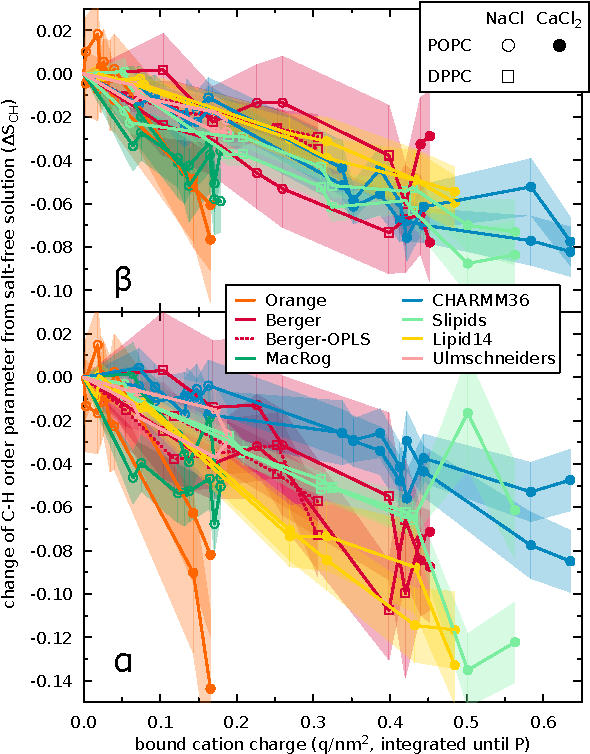
\includegraphics[width=8.8cm]{../Fig/dOP_vs_boundCationCharge_P.pdf}
  \caption{\label{electrometer}
    Change of order parameters (from salt-free solution) of the $\beta$ and $\alpha$ segments,
    $\Delta S_{\rm{CH}}^{\beta}$ and $\Delta S_{\rm{CH}}^{\alpha}$,
    as a function of bound cation charge.
    Eight MD simulation models compared; the two lines per model denote to the two hydrogens per carbon.
    The order parameters as well as the bound charge calculated separately for
    each leaflet; cations residing between the bilayer centre and the density maximum of Phosphorus
    considered bound; error bars (shaded) show standard error of mean over lipids.
   }
%\todo{Results from long CHARMM and Slipids simulations to be added.}
\end{figure}

We note that
the quantitative comparison of order parameter changes in response to bound charge should be more straightforward for
systems with charged amphiphiles fully associated in the bilayer, as the amount of bound charge
is then explicitly known in both simulations and experiments. In such a comparison
between experiments~\cite{scherer89,franzin98} and previously published Berger-model-based simulations~\cite{miettinen09},
we could not rule out
overestimation of order parameter response to bound cations (slopes $m_\alpha$ and $m_\beta$), see ESI$^\dag$.
This might, in principle, explain the overestimated order parameter 
response of the Berger model to CaCl$_2$, but not to NaCl (see discussion in ESI$^\dag$).
Since simulation data with charged amphiphiles are not available for other models,
an extended comparison with different models is left for further studies.

\begin{figure}[!h]
  \centering
  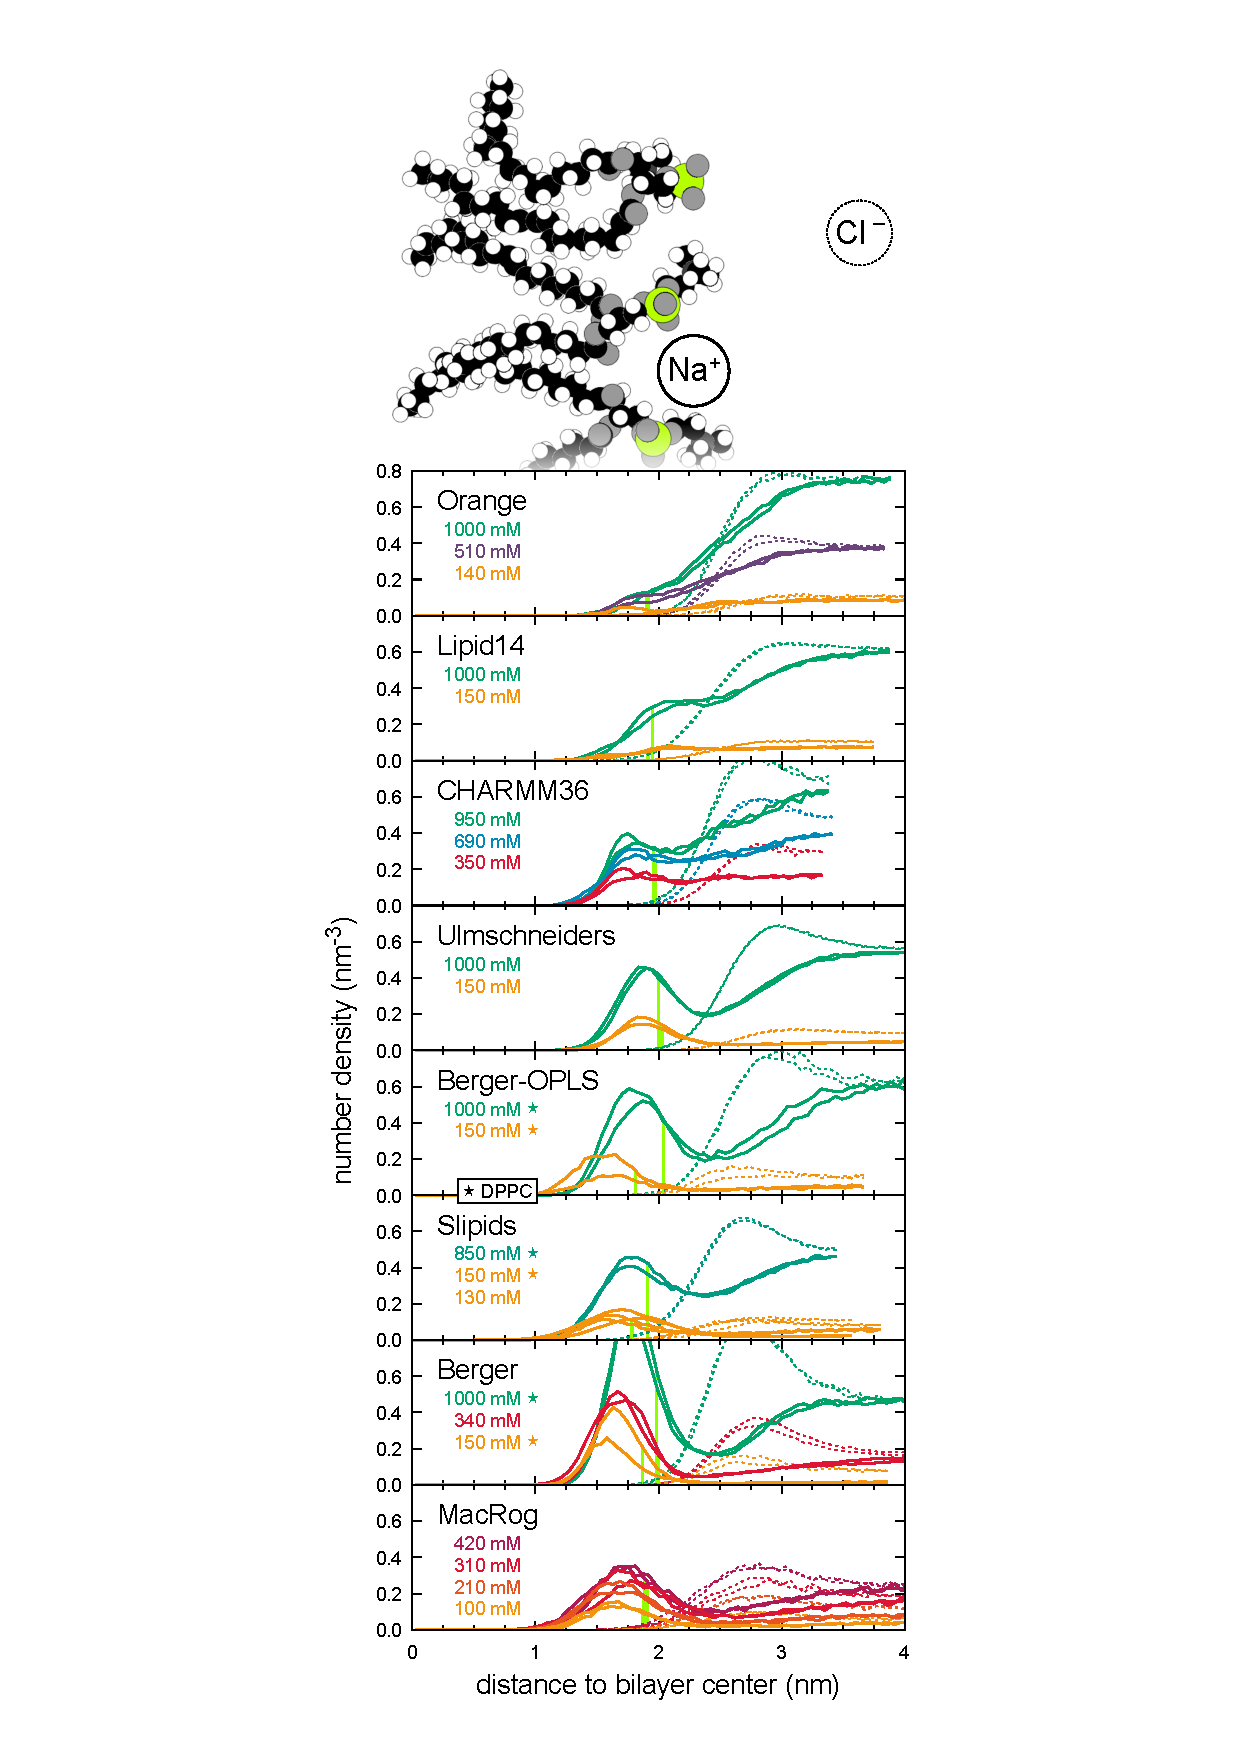
\includegraphics[width=7.595cm]{../Fig/NaDensities_withSnap.pdf}
  \caption{\label{NAdensities}
    Na$^+$ (solid line) and Cl$^-$ (dashed) distributions along the lipid bi\-layer normal from MD simulations
    at several NaCl concentrations.
    The eight MD models are ordered according to their strength of order parameter change in response to NaCl
    (Fig.~\ref{ordPions})
    from the weakest (top panel) to the strongest (bottom).
    The light green vertical lines indicate the locations of the Phosphorus maxima,
    used to define bound cations in Fig.~\ref{electrometer}.
}
\end{figure}
%
Figure~\ref{electrometer} shows that the decrease of order parameters clearly correlated with the
amount of bound cations in simulations. This is also evident from Fig.~\ref{NAdensities},
which shows the Na$^+$ density profiles of the MD models ordered according to the order parameter change 
(in Fig.~\ref{ordPions}) from the smallest (top) to the largest (bottom).
The general trend in the figure is that the Na$^+$ density peaks are 
larger for models with larger changes in order parameters,
in line with the observed correlation between cation binding and order parameter decrease in
Fig.~\ref{electrometer}.

Figure~\ref{AvsB} compares the relation between $\Delta S_{\rm{CH}}^{\beta}$ and $\Delta S_{\rm{CH}}^{\alpha}$
in experiments~\cite{akutsu81} and in MD models.
Only Lipid14 gave $\Delta S_{\rm{CH}}^{\beta}/\Delta S_{\rm{CH}}^{\alpha}$ ratio in agreement with the experimental ratio;
all other models underestimated the $\alpha$ segment order parameter decrease with bound cations with
respect to the $\beta$ segment decrease.
\begin{figure}[t]
  \centering
  \includegraphics[width=8cm]{../Fig/OrderParameterAvsB.eps}
  \caption{\label{AvsB}
    Relation between $\Delta S_{\rm{CH}}^{\beta}$ and $\Delta S_{\rm{CH}}^{\alpha}$ from experiments~\cite{akutsu81} and
    different simulation models. Solid line is $\Delta S_{\rm{CH}}^{\beta}=0.43\Delta S_{\rm{CH}}^{\alpha}$ determined for DPPC bilayer
    from $^2$H NMR experiment with various CaCl$_2$ concentrations~\cite{akutsu81}.
  }
\end{figure}

In conclusion, a clear correlation between bound cations and order parameter decrease 
was observed for all simulation models. Consequently, the molecular electrometer can 
be used to compare the cation binding affinity between experiments and simulations. 
However, we found that quantitatively the response of $\alpha$ and $\beta$ segment order parameters to bound cations in simulations 
did not generally agree with the experiments; e.g., the $\Delta S_{\rm{CH}}^{\beta}/\Delta S_{\rm{CH}}^{\alpha}$ ratio  
agreed with experiments only in the Lipid14 model (Fig.~\ref{AvsB}).
Thus, the observed overestimation of the order parameter changes with salt concentrations could, in principle, arise
from overbinding of cations or from an oversensitive lipid headgroup response to the bound cations
(see also discussion in ESI$^\dag$). 
A careful analysis with current lipid models is performed in the next section.

\begin{table*}[!p]
%\begin{sidewaystable*}[!p]
\centering
\caption{List of MD simulations. The salt concentrations calculated as 
   [salt]=N$_{\rm c} \times$[water]\,/\,N$_{\rm w}$, where [water]\,=\,55.5~M;
   these correspond the concentrations reported in the experiments by Akutsu et al.~\cite{akutsu81}.
   The lipid force fields named as in our previous work~\cite{botan15}.}\label{IONsystems}
\begin{minipage}[t]{\textwidth}
\begin{tabular}{l l l r r r r r r r c}
  %\hline
  % some footnotes are not visible in typeset-MS (pdf)
  force field for lipids / ions & lipid & salt & [salt]\,(mM) & \footnote{Number of lipid molecules}N$_{\rm l}$   &  \footnote{Number of water molecules}N$_{\rm w}$   & \footnote{Number of cations}N$_{\rm c}$  & \footnote{Simulation temperature}T (K)  & \footnote{Total simulation time}t$_{{\rm sim}}$(ns) & \footnote{Time used for analysis}t$_{{\rm anal}}$ (ns) & \footnote{Reference for simulation files}files\\
  \hline
  Berger-POPC-07\cite{ollila07a} / --  &   POPC & no & 0        & 128 			   		& 7290 & 0  & 298  & 270 & 50 & \citenum{bergerFILESpopc}  \\
  Berger-POPC-07\cite{ollila07a} / ffgmx\cite{straatsma88}  &   " & NaCl & 340 & " 		& 7202 & 44 & "  & 110 & " & \citenum{bergerPOPC340mMNaClfiles} \\
  Berger-POPC-07\cite{ollila07a} / ffgmx\cite{straatsma88}  &   " & CaCl$_2$ & 340  & " 	& 7157 & " & " & 108 & 58 &\citenum{bergerPOPC340mMCaClfiles}  \\
  %\hline
  Berger-DPPC-97\cite{marrink98} / --  &   DPPC & no & 0 & 72 						& 2880 & 0  &323  & 60 & 50 &\citenum{bergerDPPCfiles} \\
  Berger-DPPC-97\cite{marrink98} / ffgmx\cite{straatsma88}   &   " &  NaCl & 150 & " 		& "       & 8  & "  & 120 & 60 &\citenum{bergerDPPC150mMfiles} \\
  Berger-DPPC-97\cite{marrink98} / ffgmx\cite{straatsma88}   &   " & " & 1000  & " 		& 2778 & 51 & "  & " & " &\citenum{bergerDPPC1000mMfiles} \\
  \hline
  BergerOPLS-DPPC-06\cite{tieleman06} / -- &   DPPC & no & 0 & 72 					& 2880 & 0 & 323  & 120 & 60 &\citenum{bergerOPLSDPPCfiles} \\
  BergerOPLS-DPPC-06\cite{tieleman06} / OPLS\cite{aqvist90} &   " & NaCl & 150  & "	& " & 8  & "  & " & " &\citenum{bergerOPLSDPPCfiles150mMnacl} \\
  BergerOPLS-DPPC-06\cite{tieleman06} / OPLS\cite{aqvist90} &   " & " & 1000 & " 		& 2778 & 51 & "  & " & " &\citenum{bergerOPLSDPPCfiles1000mMnacl} \\
  \hline
  CHARMM36\cite{klauda10} / -- & POPC & no & 0 & 128 							& 5210 & 0 & 303 & 200 & 150 & \citenum{charmm36files} \\ % Hubert's 0CHL simu (doi: 10.5281/zenodo.14066)
  CHARMM36\cite{klauda10} / --  & " & " & 0           & 72 							& 2242 & "  & "  & 30 & 20 & \citenum{charmm36filesSHORT} \\
  CHARMM36\cite{klauda10} / CHARMM36\cite{venable13} & " & NaCl & 350   & " 		& 2085 & 13  & "  & 80 & 60 & \citenum{charmmPOPC350mMNaClfiles} \\
  CHARMM36\cite{klauda10} / CHARMM36\cite{venable13} & " & " & 690 & " 			& " & 26 & "  & 73 & " & \citenum{charmmPOPC690mMNaClfiles}   \\
  CHARMM36\cite{klauda10} / CHARMM36\cite{venable13}  & " & " & 950 & " 			& 2168 & 37 & "  & 80 & " &\citenum{charmmPOPC950mMNaClfiles}  \\
  CHARMM36\cite{klauda10} / CHARMM36 & " & CaCl$_2$ & 350  & 128 				& 6400 & 35 & "  & 200  & 100 & \citenum{charmmPOPC350mMCaClfiles}  \\
  CHARMM36\cite{klauda10} / CHARMM36 & " & " & 450  & 200 					& 9000 & 73 & 310  & 2000  & " & \citenum{charmmPOPC450mMCaClfiles}  \\
  CHARMM36\cite{klauda10} / CHARMM36 & " & " & 670  & 128 					& 6400 & 67 & 303  & 200  & 120 & \citenum{charmmPOPC670mMCaClfiles}  \\  
  CHARMM36\cite{klauda10} / CHARMM36 & " & " & 1000 & " 						& " & 100 & " & "  & 100 & \citenum{charmmPOPC1000mMCaClfiles}  \\
  %\hline
  CHARMM36\cite{klauda10} / -- & DPPC & no & 0  & 128 							& 8000 & 0 & 323  & 170 & 150 & --  \\
  CHARMM36\cite{klauda10} / Yoo\cite{yoo16}  & " & CaCl$_2$ & 430   & " 			& 7760 & 60 & "  & 200 & 170 & --  \\
  CHARMM36\cite{klauda10} / Yoo\cite{yoo16}  & " & " & 890  & " 					& 7520 & 120 & "  & " & " & --  \\
  \hline
  MacRog\cite{maciejewski14} / -- & POPC & no & 0 & 128 							& 6400 & 0 & 310 & 400& 200 & \citenum{macrogCHOLfiles}  \\ % Matti's 0CHL simu (doi: 10.5281/zenodo.13877)
  MacRog\cite{maciejewski14} / -- & " & " & 0 & 288 								& 14400 & " & " & 90 & 40  & \citenum{macrogdehydFILES}  \\  
  MacRog\cite{maciejewski14} / OPLS\cite{aqvist90}  & " & NaCl & 100  & " 			& 14554 & 27 & " & " &50  & \citenum{macrogIONfiles} \\
  MacRog\cite{maciejewski14} / OPLS\cite{aqvist90}  & " & " & 210  & " 				& 14500 & 54 & " & " & "  & "  \\
  MacRog\cite{maciejewski14} / OPLS\cite{aqvist90}  & " & " &  310 & " 				& 14446 & 81 & " & " & "  & " \\
  MacRog\cite{maciejewski14} / OPLS\cite{aqvist90}  & " & " &  420 & " 				& 14392 & 108 & " & " & "  & "  \\
  \hline
  Orange / --            			& POPC & no & 0 & 72 	& 2880 & 0 & 298 & 60 & 50 & \citenum{orangePOPCfiles}  \\
  Orange / OPLS\cite{aqvist90}	&   " & NaCl & 140  & " 	& 2866 & 7 & " & 120 & 60 &\citenum{orangePOPC140mMNaClfiles}  \\
  Orange / OPLS\cite{aqvist90} 	&   " & " & 510 & " 		& 2802 & 26 & " & " & 100 &\citenum{orangePOPC510mMNaClfiles}   \\
  Orange / OPLS\cite{aqvist90} 	&   " & " & 1000 & " 		& 2780 & 50 & " & " & 80 & \citenum{orangePOPC1000mMNaClfiles} \\
  %\hdashline
  Orange / OPLS &   " & CaCl$_2$ & 510  & " 			& 2802 & 26 & " & " & 60 & \citenum{orangePOPC510mMCaClfiles}  \\
  \hline
  Slipids\cite{jambeck12b} / --  &   POPC & no & 0 & 128 					& 5120 & 0 & 310 & 200 & 150 &~\citenum{slipidsFILESpopc}  \\
  Slipids\cite{jambeck12b} / AMBER\cite{smith94}  &  " & NaCl & 130 & 200 	& 9000 & 21 & " & 105 & 100 &~\citenum{slipidsFILESpopc130mMnaclSD}  \\
  Slipids\cite{jambeck12b} / AMBER\cite{aqvist90}  &  "& CaCl$_2$ & 450  & " 	& "  & 73 & " & 2000 & " &~\citenum{slipidsFILESpopc450mMcacl}  \\
  %\hline
  Slipids\cite{jambeck12} / -- &   DPPC & no & 0 & 128 		& 3840 & 0 & 323 & 150 & 100 &~\citenum{slipidsFILES}  \\
  Slipids\cite{jambeck12} / AMBER\cite{beglov94,roux96} &   " & NaCl & 150  & 600 	& 18000 & 49 & " & 100 & 40 &--  \\
  Slipids\cite{jambeck12} / AMBER\cite{beglov94,roux96} &   " & " & 850 & 128 		& 3726 &  57 & " & 205 & 200 & \citenum{slipidsFILESdppc}  \\
  Slipids\cite{jambeck12} / AMBER\cite{beglov94,roux96} &   " & " & 1750 & " 		& 3612 &  114 & " & 105 & 100 & "  \\
  Slipids\cite{jambeck12} / AMBER\cite{beglov94,roux96} &   " & " & 2570 & " 		& 3514 &  163 & " & " & " & "  \\
  \hline
  Lipid14~\cite{dickson14} / --                        &   POPC & no 		& 0		& 128	& 5120 	& 0 & 298 & 205 & 200 &~\citenum{lipid14POPC0mMNaClfiles}  \\
  Lipid14~\cite{dickson14} / AMBER\cite{aqvist90}   &   " & NaCl & 150	& " 		& " 		& 12 & " & " & " &~\citenum{lipid14POPC150mMNaClfiles}  \\
  Lipid14~\cite{dickson14} / AMBER\cite{aqvist90}   &   " & " 	& 1000 	& " 		& " 		& 77 & " & " & " &~\citenum{lipid14POPC1000mMNaClfiles}  \\
  Lipid14~\cite{dickson14} / AMBER\cite{aqvist90}   &   " & CaCl$_2$ & 350 & " 		& 6400 	& 35 & " & 200 & 100 &~\citenum{lipid14POPC350mMCaClfiles}  \\
  Lipid14~\cite{dickson14} / AMBER\cite{aqvist90}   &   " & " 	& 1000 	& " 		& " 		& 100 & " & " & " &~\citenum{lipid14POPC1000mMCaClfiles}  \\
  \hline
  Ulmschneiders~\cite{Ulmschneider09} / --                           		& POPC 	& no 		& 0		& 128 & 5120 	& 0 & 298 & 2$\times$205 & 2$\times$200 &~\citenum{ulmschneiderPOPC0mMNaClfiles}  \\
  Ulmschneiders~\cite{Ulmschneider09} / OPLS\cite{aqvist90}	&   " 		& NaCl 	& 150 	& " 	  & " 		& 12 & " & 205 & 200 &~\citenum{ulmschneiderPOPC150mMNaClfiles}  \\
  Ulmschneiders~\cite{Ulmschneider09} / OPLS\cite{aqvist90}	&   " 		& " 		& 1000  	& " 	  & " 		& 77 & " & " & " &~\citenum{ulmschneiderPOPC1000mMNaClfiles}  \\
\end{tabular}
\end{minipage}
%\end{sidewaystable*} 
\end{table*}







\subsection{Cation binding in different simulation models}

The order parameter changes (Fig.~\ref{ordPions}) and density distributions (Fig.~\ref{NAdensities})
demonstrated significantly different Na$^+$ binding affinities in different simulation models.
The best agreement with experiments (lowest $\Delta S_\mathrm{CH}^\alpha$ and $\Delta S_\mathrm{CH}^\beta$) was observed for the three models (Orange, Lipid14, CHARMM36; see Fig.~\ref{ordPions}) that predicted the lowest Na$^+$ densities 
near the bilayer (Fig.~\ref{NAdensities}).
All the other models clearly overestimated the choline order parameter 
responses to NaCl (Fig.~\ref{ordPions}) --- and notably
the strength of the overestimation was clearly linked to the strength of the
Na$^+$ binding affinity (compare Figs.~\ref{ordPions} and~\ref{NAdensities}),
which leads us to conclude that Na$^+$ binding affinity was overestimated in all these models.

As in the best three models the order parameter changes with NaCl were small ($<0.02$),
the achieved statistical accuracy did not allow us to conclude 
which of the three had the most realistic Na$^+$ binding affinity,
especially at physiological NaCl concentrations ($\sim$\,150\,mM) 
relevant for most applications. 
The overestimated binding in the other models raises questions concerning the quality of predictions from these models when NaCl is present.
%\todo{It has been suggested that we should add references here. The problem is that there are a lot of them and
%it is difficult to choose which ones to pick. Any opinions?} {\it Mention that there are many (hundreds?) of them in Web of Science? -markus.}
%OLLILA: I have left this like it is.
Especially interactions between charged molecules and the bilayer might be significantly
affected by the strong Na$^+$ binding, which gives the otherwise neutral bilayer an effective positive charge.

Significant Ca$^{2+}$ binding affinity for phosphatidylcholine bilayers at sub-molar concentrations  
is agreed on in the literature~\cite{akutsu81,altenbach84,cevc90,tocanne90}, however, several
details remain under discussion. Simulations suggest that Ca$^{2+}$ binds to lipid carbonyl
oxygens with a coordination number of 4.2~\cite{bockmann04}, while interpretation of NMR and 
scattering experiments suggest that one Ca$^{2+}$ interacts mainly with the choline 
groups~\cite{hauser76,hauser78,herbette84} of two phospholipid molecules~\cite{altenbach84}. 
A simulation model correctly reproducing the order parameter changes would resolve the discussion
by giving atomistic resolution interpretation for the experiments.

As a function of CaCl$_2$ concentration, all models but one (CHARMM36 with the recent heptahydrated Ca$^{2+}$ by Yoo et al.~\cite{yoo16})
overestimated the order parameter decrease (Fig.~\ref{ordPions}),
which according to the molecular electrometer indicates too strong Ca$^{2+}$ binding.
(We note that while this is the most likely scenario for the models that overestimated changes in both order parameters,
for CaCl$_2$ it is possible also that the headgroup response is oversensitive to
bound cations, see ESI$^\dag$.)
In CHARMM36 with the heptahydrated Ca$^{2+}$ by Yoo et al.~\cite{yoo16},
$\Delta S_\mathrm{CH}^\beta$ was overestimated  but $\Delta S_\mathrm{CH}^\alpha$ underestimated (Fig.~\ref{ordPions}),
in line with the $\Delta S_{\rm{CH}}^{\beta}/\Delta S_{\rm{CH}}^{\alpha}$ ratio
in CHARMM36 being larger than in experiments (Fig.~\ref{AvsB}). As we do not know whether $\Delta S_{\rm{CH}}^{\beta}$ or $\Delta S_{\rm{CH}}^{\alpha}$
was more realistic, we cannot conclude whether Ca$^{2+}$ binding was too strong or too weak in CHARMM36.
This could be resolved by comparing against experimental data with a known amount of bound charge 
(e.g., amphiphilic cations~\cite{scherer89,franzin98}), however, such simulation data are not
currently available.

The density distributions with CaCl$_2$ showed significant
Ca$^{2+}$ binding in all models (Fig.~\ref{CAdensitiesCLEAR}), however, some differences occurred in details.
The Berger model predicted deeper penetration (density maximum at $\sim$\,1.8\,nm) compared
to other models ($\sim$\,2\,nm); the latter value is probably more realistic 
as $^1$H~NMR and neutron scattering data indicate that Ca$^{2+}$ interacts mainly with the 
choline group~\cite{hauser76,hauser78,herbette84,cevc90}. In CHARMM36 (but not in Slipids) practically all Ca$^{2+}$
ions present in the simulation bound the bilayer within 2\,$\mu$s (Fig.~\ref{CAdensitiesCLEAR} and ESI$^\dag$), which hints
that the Ca$^{2+}$ binding affinity of CHARMM36 is among the strongest of these models.
%The difference is not as clear in Fig.~\ref{ordPions} because $\alpha$ carbon order parameters 
%are the least sensitive to bound charge in CHARMM36 (Fig.~\ref{electrometer}).
\begin{figure}[!h]
  \centering
  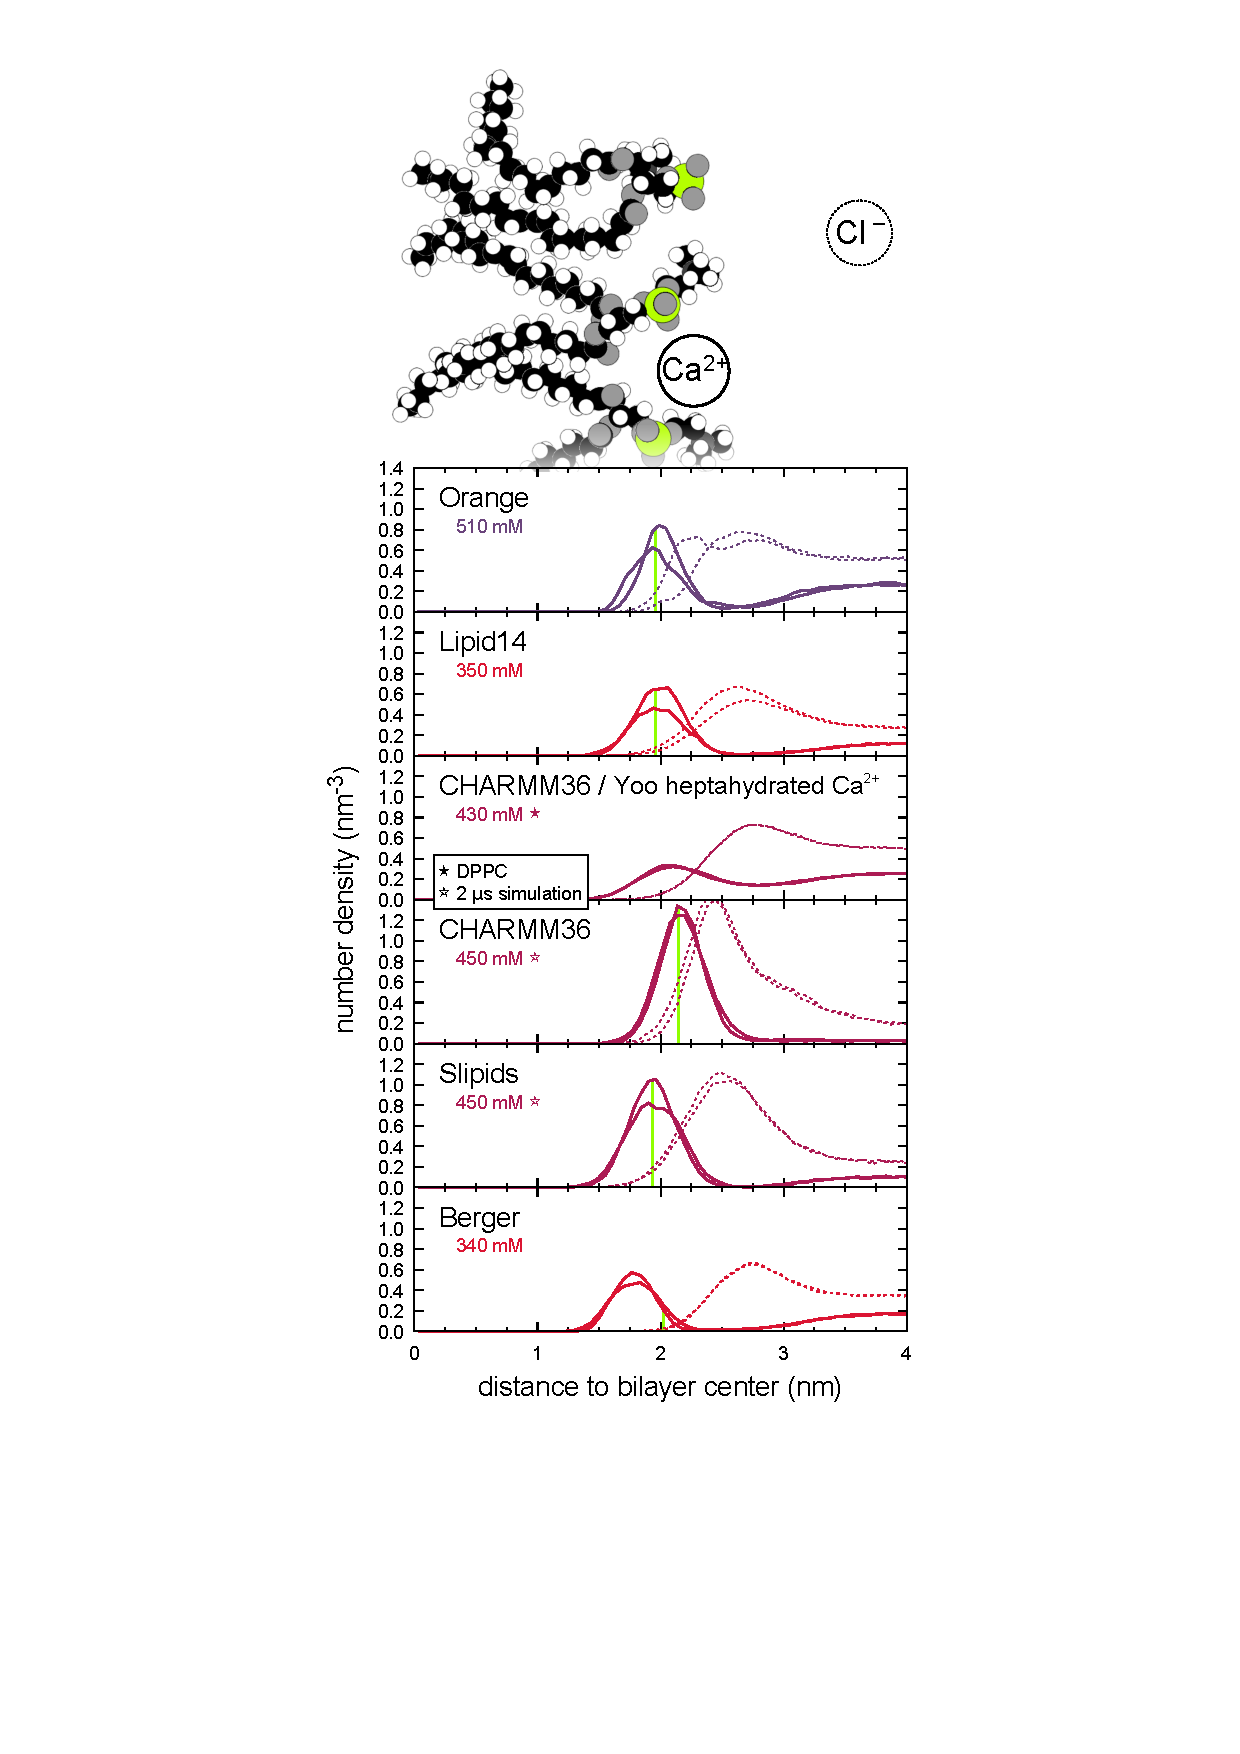
\includegraphics[width=7.6cm]{../Fig/CaDensities_withSnap.pdf}
  \caption{\label{CAdensitiesCLEAR}
    Ca$^{2+}$ (solid line) and Cl$^-$ (dashed) distributions along the lipid bi\-layer normal from MD simulations.
    For clarity, only one CaCl$_2$ concentration per MD model is shown;
    see ESI$^\dag$ for a plot including all the available concentrations.
    The light green vertical lines indicate the locations of the Phosphorus maxima,
    used to define bound cations in Fig.~\ref{electrometer}.
  }
\end{figure}

The origin of inaccuracies in lipid--ion interactions and binding affinities is far from clear.
Potential candidates are, e.g., discrepancies in the ion models~\cite{hess06,chen07,Reif13},
incomplete treatment of electronic polarizability~\cite{leontyev11}, and inaccuracies in the lipid headgroup 
description~\cite{botan15}.

Considering the ion models, Cordomi et al.~\cite{cordomi09} showed the Na$^+$ binding affinity to decrease when ion radius is increased;
however, in their DPPC bilayer simulations (with the OPLS-AA force field~\cite{jorgensen96}) even the largest Na$^+$ radii still resulted in significant binding.
In our results, the Slipids force field gave essentially similar binding affinity with 
ion parameters from Refs.~\citenum{smith94} and~\citenum{beglov94,roux96} (Fig.~\ref{NAdensities}). Further, compensation of missing electronic 
polarizability by scaling the ion charge~\cite{kohagen16,leontyev11} reduced Na$^+$ binding in Berger, 
Berger-OPLS and Slipids, but not enough to reach agreement with experiments (ESI$^\dag$). 
The charge-scaled Ca$^{2+}$ model~\cite{kohagen14} slightly reduced binding in CHARMM36, but did not have 
significant influence in Slipids (ESI$^\dag$).
The heptahydrated Ca$^{2+}$ ions by Yoo et al.~\cite{yoo16} significantly reduced Ca$^{2+}$ binding in CHARMM36 (Fig.~\ref{CAdensitiesCLEAR}), however, the
model must be further analysed to fully interpret the results.

The lipid models may also have a significant influence on ion binding behaviour.
For example, the same ion model and non-bonded parameters are used in Orange and Berger-OPLS~\cite{tieleman06},
but while Na$^+$ ion binding affinity appeared realistic in Orange, it was significantly overestimated 
in Berger-OPLS (Fig.~\ref{NAdensities}). However, realistic Na$^+$ binding does not automatically imply
realistic Ca$^{2+}$ binding (see Orange, Lipid14, and CHARMM36 in Fig.~\ref{ordPions}) or realistic choline
order parameter response to bound charge (see Orange and CHARMM36 in Fig.~\ref{AvsB}).
It should also be noted that the low binding affinity of Na$^+$ in CHARMM36 is due to 
the additional repulsion (NBFIX~\cite{venable13}) added between the sodium ions and lipid oxygens (ESI$^\dag$),
and that in the Ca$^{2+}$ model by Yoo et al.~\cite{yoo16} the calcium is forced to be solvated solely by water.
Altogether, our results indicate that probably both, lipid and ion force field parameters, need improvement to 
correctly predict the cation binding affinity, and the associated structural changes.


\section{Conclusions}
In accordance with the molecular electrometer~\cite{brown77,akutsu81,altenbach84,seelig87,scherer89},
cation binding to lipid bilayers was accompanied with a decrease in the C--H order parameters of the PC head group $\alpha$ and $\beta$ carbons 
in all the simulation models tested (Fig.~\ref{electrometer}) --- despite of the known inaccuracies 
in the actual atomistic resolution structures~\cite{botan15}. Hence, the molecular electrometer allowed a direct comparison
of Na$^+$ binding affinity between simulations and noninvasive NMR experiments.
The comparison revealed that most models overestimated Na$^+$ binding; only Orange, Lipid14, and CHARMM36 
predicted realistic binding affinities. None of the tested models had the accuracy required to interpret
the Ca$^{2+}$:lipid stoichiometry or the induced structural changes with atomistic resolution.

Taken together, our results corroborate the pre-2000 view that at sub-molar concentrations, in contrast to Ca$^{2+}$ and other multivalent ions~\cite{eisenberg79,akutsu81,altenbach84,tatulian87,cevc90,tocanne90,clarke99,binder02,pabst07,filippov09},
Na$^+$ and other monovalent ions (except Li$^+$) do not specifically bind to phospholipid bilayers.
Concerning the interpretation of existing experimental data, our work supports Cevc's view~\cite{cevc90}
that the observed small shift in phase transition temperature is not indicative of Na$^+$ binding.
Further, our findings are in line with the noninvasive NMR spectroscopy work of Filippov et al.~\cite{filippov09} 
that proved the results of Refs.~\citenum{bockmann03,vacha09a,harb13} to be explainable by direct interactions between Na$^+$ ions and fluorescent probes.
Finally, as spectroscopic methods are in general more sensitive to atomistic details in fluid-like environment than AFM, our work indirectly suggests that the ion 
binding reported from AFM experiments on fluid-like lipid bilayer systems~\cite{manyes05,manyes06,fukuma07,ferber11,morata12} might be confounded with other physical features of the system.
%\todo{This feels like a detached comment\ldots Could we back this claim up, or rephrase? I mean, now it sounds a bit like we came to conclude based on our simulations that the AFM resolution is not enough. \\
%OLLILA: Rephrasing is welcomed. In the the end, my justification for this comment is that spectrocopy is in general more reliable for atomistic resolution information than AFM in fluid--like environment. Also, I think that the AFM data supporting Na binding is quite indirect and can be interpreted in many ways but full discussion about this would be quite complicated I think. }}
Concerning contradictions in MD simulation results, we reinterpret the strong Na$^+$ binding as an artefact of several simulation models, e.g., the Berger model used in Refs.~\citenum{bockmann03,bockmann04}.

The artificial specific Na$^+$ binding in MD simulations may lead to doubtful results, as it effectively results in a
positively charged phosphatidylcholine lipid bilayer even at physiological NaCl concentrations.
Such a charged bilayer will have distinctly different interactions with charged objects than what a (more realistic)
model without specific Na$^+$ binding would predict. Furthermore, the overestimation of binding affinity may
extend from ions to other positively charged objects, say, membrane protein segments. This would affect
lipid--protein interactions and could explain, for example, certain contradicting results on electrostatic interactions 
between charged protein segments and lipid bilayers~\cite{arkhipov13,kaszuba15}. In conclusion, 
more careful studies and model development on lipid bilayer--charged object interactions are urgently
called for to make molecular dynamics simulations directly usable in a physiologically relevant
electrolytic environment. 
%I have changed back to ''directly usable'' because simulation can be used also for intepretation
%besides of prediction. Also I want to keep word directly because simulations might be usable
%but only with very careful analysis. 

% Seelig's 1987 paper where the concept molecular electrometer is first mentioned stresses that it is not limited to ion binding, but can be used to study "any process that modifies the electrical properties of the membrane surface". Maybe we should repeat that quote to emphasize that molecular electrometer is a general means to assess the membrane electrical responses. Currently many people use additional molecular probes to measure electric responses, yet the molecular electrometer is a "non-invasive, non-perturbing" alternative.

This work was done as a fully open collaboration, using
\url{nmrlipids.blogspot.fi} as the communication platform. All the
scientific contributions were communicated publicly through
this blog or the GitHub repository \cite{githubIONpaper}. % \url{https://github.com/NMRLipids/lipid_ionINTERACTION}.
All the related content and data are available at Ref.~\citenum{githubIONpaper}. %\url{https://github.com/NMRLipids/lipid_ionINTERACTION}.
%Befor publication I will create Zenodo link from GitHub repo which will be cited here.

%This work has been, and will be, progressed and discussed through the blog \url{nmrlipids.blogspot.fi}, through which 
%everyone is invited to join the discussion and make contributions. 
%The manuscript will be eventually submitted to an appropriate scientific journal. 
%Everyone who has contributed to the work through the blog will be offered 
%coauthorship. For more details see \url{nmrlipids.blogspot.fi}.   

{\bf Acknowledgements: }
AC and VSO wish to thank the Research Computing Service at UEA for access to the High Performance Computing Cluster; VSO acknowledges the Engineering and Physical Sciences Research Council in the UK for financial support (EP/L001322/1).
%
MG acknowledges financial support from Finnish Center of International Mobility (Fellowship TM-9363).
%
J. Melcr acknowledges computational resources provided by the CESNET LM2015042 and the CERIT Scientific Cloud LM2015085 projects under the program ''Projects of Large Research, Development, and Innovations Infrastructure''.
%
MSM acknowledges financial support from the Volkswagen Foundation (86110).
%
LM acknowledges funding from the Institut National de la Sante et de la Recherche Medicale (INSERM).
%
OHSO acknowledges Tiago Ferreira for very useful discussions, the Emil Aaltonen foundation for financial support, Aalto Science-IT project and CSC-IT Center for Science for computational resources. 

\bibliography{refs} %You need to replace "rsc" on this line with the name of your .bib file
\bibliographystyle{rsc} %the RSC's .bst file


\end{document}
